\begin{minipage}{.65\textwidth}
โดยทั่วไปแล้วการเคลื่อนที่แบบวงกลม จะมีแรงเกี่ยวข้องอย่างน้อย  2  แรงเสมอ  ได้แก่
\begin{itemize}[leftmargin=*]
	\item[1)] \textbf{แรงหนีศูนย์กลาง}  จะพยายามผลักวัตถุออกไปจาก\\วงกลมอยู่ตลอดเวลา
	\item[2)] \textbf{แรงเข้าสู่ศูนย์กลาง}   จะพยายามดึงวัตถุเข้าสู่จุด\\ศูนย์กลางของวงกลมเสมอ	
\end{itemize}
\end{minipage} \hfill
\begin{adjustbox}{valign=c} 
    \begin{minipage}[c]{.3\linewidth}
        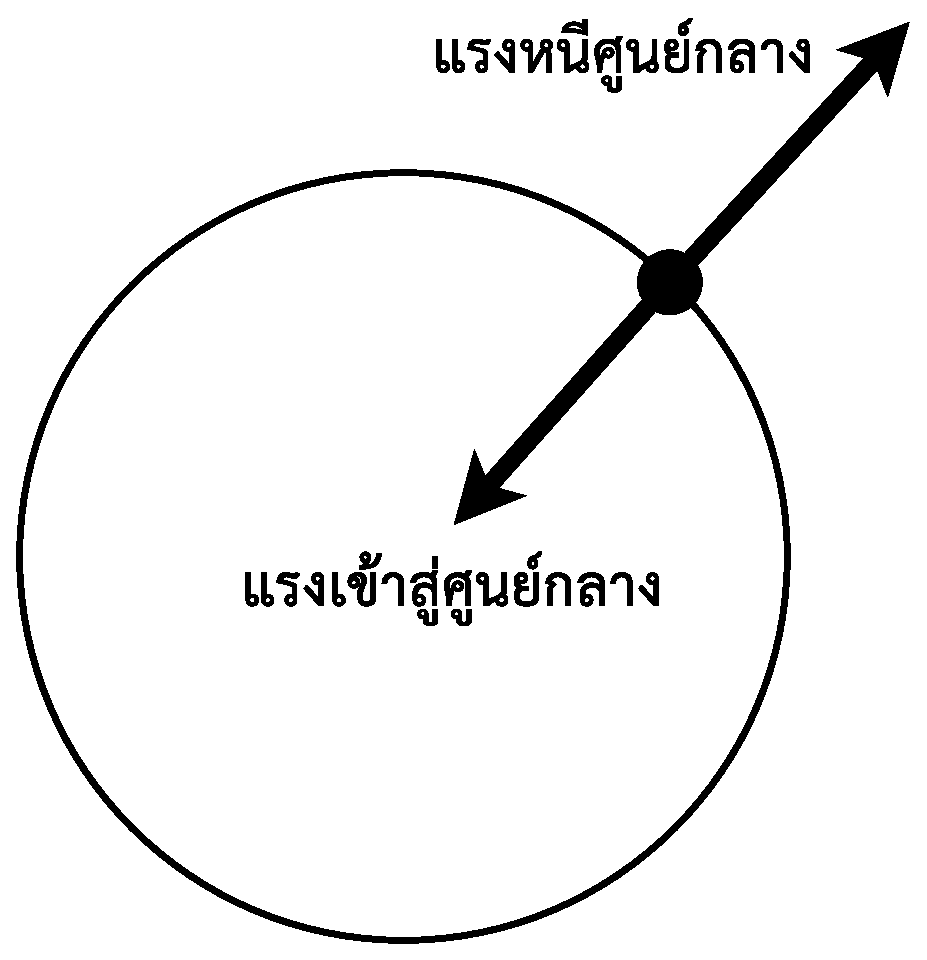
\includegraphics[width=\linewidth]{content-12.eps}
    \end{minipage}
\end{adjustbox}
\tcblower
ปกติแล้วแรงทั้งสองนี้จะมีขนาดเท่ากัน แต่มีทิศตรงกันข้ามดังรูป   ทั้งนี้เพื่อให้วัตถุอยู่ในภาวะสมดุลของแรงนั่นเอง แรงเข้าสู่ศูนย์กลางของการเคลื่อนที่แต่กรณีอาจมีลักษณะที่แตกต่างกันไป   \textbf{ตัวอย่างเช่น}
\begin{center}
\begin{minipage}{.6\textwidth}
การเคลื่อนที่ของวัตถุที่ผูกไว้ด้วยเชือกแล้วเหวี่ยงให้เคลื่อนที่เป็นวงกลม       แรงที่ทำหน้าที่เป็นแรงเข้าสู่ศูนย์กลางคือแรงดึงเชือก
\end{minipage} \hfill
\begin{adjustbox}{valign=c} 
    \begin{minipage}[t]{.35\linewidth}
        \includegraphics[width=\linewidth]{content-12-1.jpg}
    \end{minipage}
\end{adjustbox}
\end{center}

\begin{center}
\begin{minipage}{.6\textwidth}
การเลี้ยวโค้งบนถนนของรถ	แรงที่ทำหน้าที่เป็นแรงเข้าสู่ศูนย์กลางคือแรงเสียดทานระหว่างยางรถกับพื้นถนน
\end{minipage} \hfill
\begin{adjustbox}{valign=c} 
    \begin{minipage}[t]{.35\linewidth}
        \includegraphics[width=\linewidth]{content-12-4.jpg}
    \end{minipage}
\end{adjustbox}
\end{center}

\begin{center}
\begin{minipage}{.6\textwidth}
การโคจรของดวงจันทร์รอบโลกแรงที่ทำหน้าที่เป็นแรงเข้าสู่ศูนย์กลางคือแรงดึงดูดที่โลกดูดดวงจันทร์ไว้นั่นเอง
\end{minipage} \hfill
\begin{adjustbox}{valign=c} 
    \begin{minipage}[t]{.35\linewidth}
        \includegraphics[width=\linewidth]{content-12-2.jpg}
    \end{minipage}
\end{adjustbox}
\end{center}

\begin{center}
\begin{minipage}{.6\textwidth}
การเคลื่อนที่ของรถไฟเหาะตีลังกา    หากรถอยู่ที่จุดสูงสุดของราง     แรงที่ทำหน้าที่เป็นแรงเข้าสู่ศูนย์กลางคือน้ำหนักรถไฟรวมกับแรงดันของพื้นราง    แต่ถ้ารถอยู่ที่จุดต่ำสุดของรางแรงที่ทำหน้าที่เป็นแรงเข้าสู่ศูนย์กลางคือน้ำหนักรถไฟอย่างเดียวดังแสดงในรูป
\end{minipage} \hfill
\begin{adjustbox}{valign=c} 
    \begin{minipage}[t]{.35\linewidth}
        \includegraphics[width=\linewidth]{content-12-3.jpg}
    \end{minipage}
\end{adjustbox}
\end{center}
